\documentclass[12pt]{article}
\usepackage{listings}
\usepackage{url}
\usepackage{comment}
\usepackage{graphicx}


\begin{document}


%% command definition

\newcommand{\todo}[1]
{\paragraph{}\textbf{TODO}: #1}

\lstnewenvironment{vhdl}
{\lstset{language=VHDL, basicstyle=\tiny, frame=single}}{}

\lstnewenvironment{sh}
{\lstset{frame=single}}{}

\newcommand{\longurl}[2]
{\url{#1#2}}

\newcommand{\longlongurl}[3]
{\url{#1#2#3}}

\IfFileExists{version.tex}
{\input{version.tex}}{\newcommand{\version}{none}}


%% block contents passed to tex preprocessor
%% ignored when processed directly by latex
%% use with \begin{texpp} \end{texpp}
\excludecomment{texpp}


%%
%% document start here

\title{Absolute encoder package}
\author{Fabien Le Mentec \\ lementec@esrf.fr}
\date{\small{version: \version}}
\maketitle


\newpage
\setcounter{tocdepth}{2}
\tableofcontents


%%
\newpage
\section{Description}

\subsection{Overview}
\paragraph{}
The absenc\_pkg implements components for absolute encoder masters and
slaves.

\paragraph{}
The term \textit{master} refers to the component driving the clock, or at
least initiating the data transfer. It is often referred to as the
\textit{controller}. The term \textit{slave} refers to the actual encoder
device.

\paragraph{}
This package is optimized for applications that can be dynamically configured
to use one amongst different types of interfaces at a particular time. As much
as possible, resources that can be shared across interfaces are factorized
(counters, comparators, shift registers ...) and accessed through a multiplexer.
However, and in order to avoid penalizing simpler applications, static
configuration allows to exclude resources associated with an unused interface.
\begin{center}
  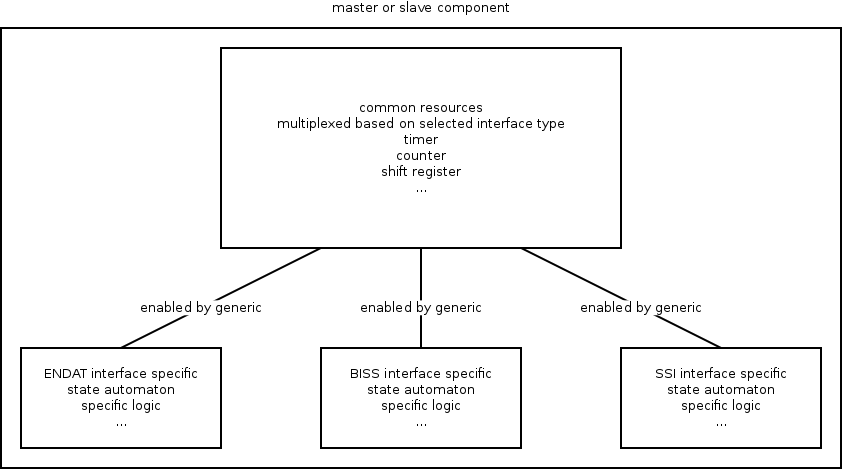
\includegraphics[width=0.8\textwidth]{./dia/arch/main.png}
\end{center}

\paragraph{}
The master implements the following data conversion pipeline:
\begin{center}
  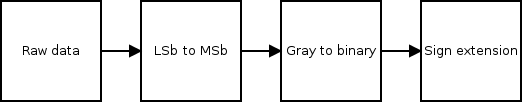
\includegraphics[width=0.5\textwidth]{./dia/master_pipeline/main.png}
\end{center}

\subsection{Features and limitations}
\begin{itemize}
\item Applicable to all
  \begin{itemize}
  \item master and slave modes,
  \item configurable master clock frequency,
  \item configurable data length (up to 48 bits),
  \item static timeout.
  \end{itemize}
\item ENDAT
  \begin{itemize}
  \item send position mode version 2.1 only,
  \item no CRC check.
  \end{itemize}
\item BISS
  \begin{itemize}
  \item point to point configuration only,
  \item no interleaved bit support (ie. CDS, CDM).
  \end{itemize}
\item SSI
   \begin{itemize}
   \item optional gray data coding (master only),
   \item optional parity bit (not checked).
   \end{itemize}
\item HSSL
   \begin{itemize}
   \item reader only,
   \item no \textit{master} or \textit{slave} interface.
   \end{itemize}
\end{itemize}


\subsection{Tested hardware}
\paragraph{}
The package has been tested with the following masters:
\begin{itemize}
  \item ICEPAP ESRF motor controller (SSI),
  \item PEPU ESRF encoder processor (SSI, BISS, ENDAT),
  \item MUSST ESRF sequencing platform (SSI),
  \item Aerotech Soloist CP controller (BISS, ENDAT).
\end{itemize}

\paragraph{}
The package has been tested with the following slaves:
\begin{itemize}
  \item PEPU ESRF encoder processor (SSI, BISS, ENDAT),
  \item Kubler sendix 5863 SIL BISS encoders,
  \item IVO industries GA241 SSI encoders,
  \item Heidenhain ROQ 425 512 ENDAT encoders,
  \item Heidenhain ROQ 437 2048 ENDAT encoders.
\end{itemize}


\subsection{Performances}

\subsubsection{EnDAT}
\paragraph{}
The following tests were done using a ROQ425 EnDAT 25 bits encoder. The master
clock frequency was made variable, along with the cable length thus the signal
propagation time.

\begin{center}
  \begin{tabular}{ | c | c | c |}
    \hline
    cable length & propagation delay & validated frequency \\ \hline
    3.5m         & 141ns             & 2.77MHz             \\ \hline
    20m          & 392ns             & 961KHz              \\ \hline
    30m          & 478ns             & 961KHz              \\ \hline
    50m          & 709ns             & 595KHz              \\ \hline
    \end{tabular}
\end{center}


%%
\newpage
\section{Interfaces}

\begin{texpp}
Texpp.include(
 kind = 'interface',
 path = '../src/absenc_pkg.vhd',
 name = 'master'
)
\end{texpp}

\begin{texpp}
Texpp.include(
 kind = 'interface',
 path = '../src/absenc_pkg.vhd',
 name = 'slave'
)
\end{texpp}


%%
\newpage
\section{Examples}

\begin{texpp}
Texpp.include(
 kind = 'example',
 path = '../sim/common/main.vhd',
 name = 'master'
)
\end{texpp}

\begin{texpp}
Texpp.include(
 kind = 'example',
 path = '../sim/common/main.vhd',
 name = 'slave'
)
\end{texpp}


\end{document}
